%%%%%%%%%%%%%%%%%%%%%%%%%%%%%%%%%%%%%%%%%%%%%%%%%%%%%%%%%%%%%%%%%%%%%%%%%%%%%
%%%  Publishing and Consuming Government Linked Data on the Semantic Web  %%%
%%%%%%%%%%%%%%%%%%%%%%%%%%%%%%%%%%%%%%%%%%%%%%%%%%%%%%%%%%%%%%%%%%%%%%%%%%%%%

\documentclass[a4paper,11pt]{report}
%\usepackage[latin1]{inputenc}
\usepackage{chngcntr}
\usepackage[english]{babel}
\usepackage{graphicx} 
\usepackage{pdfpages}
\usepackage{fancyvrb}
\usepackage{pdflscape}
\usepackage{fancyhdr}
\usepackage[utf8]{inputenc}
\usepackage{amssymb}
\pagestyle{fancy}
\setcounter{tocdepth}{3}
\usepackage{tabularx}
\usepackage{url}
\usepackage{listings}
\bibliographystyle{unsrt}


%\fancyhead[CO,CE]{---MidTerm Report--}
\fancyhead[RO, LE] {\thepage}
\renewcommand{\headrulewidth}{0.4pt}
\renewcommand{\footrulewidth}{0.4pt}

%DO NOT restart my footnotes please
\counterwithout{footnote}{chapter}
%%%%%%%%%%%%%%%%%%%%%%%%%%%%%%%
%%%  Beginning of document  %%%
%%%%%%%%%%%%%%%%%%%%%%%%%%%%%%%

\begin{document}

\begin{titlepage}
\begin{center}

\includegraphics[width=5cm]{EURECOM_logo_quadri}
\\[3cm]
\textbf{\Huge{MidTerm Report}}
\\[4cm]
\textbf{\textsc{\LARGE{Publishing and Consuming Government Linked Data on the Semantic Web}}}
\\[0.5cm]
\LARGE{Ghislain Auguste Atemezing}
\\[0.5cm]
\small{EURECOM-Multimedia Communications}
\\
\large{Institut Mines-T\'{e}l\'{e}com}
\\
\large{December 19th, 2012}
\\[5cm]
\columnsep3cm
\begin{tabular}{p{8cm} p{8.5cm}}
\small{\textbf{Supervisor:}\newline
Rapha\"el Troncy} 
&
\small{\textbf{EURECOM\newline Multimedia Department}}
\end{tabular}
\end{center}
\end{titlepage}

 \tableofcontents

%%%%%%%%%%%%%%%%%%%
%%%   Abstract  %%%
%%%%%%%%%%%%%%%%%%%

\chapter*{Abstract}
\addcontentsline{toc}{chapter}{Abstract}

The need for geolocation is crucial for many applications for both human and software agents. More and more data is opened and interlinked using Linked Data principles, and it is worth modeling geographic data efficiently by reusing as much as possible from existing ontologies or vocabularies that describe both the geospatial features and their shapes. Our aim is to contribute to the actual efforts in representing geographic objects with attributes such as location, points of interest (POI), and addresses in the web of data, with a special focus on the French territory.
As we publish data in RDF graphs, we are also aware of making them useful for the users. For that, we not only develop innovative applications to show up the value of data visualizations, but rather go beyond it. The challenge is to detect patterns to automatically develop an application using adequate visualization widgets in an affordable effort.  

%%%%%%%%%%%%%%%%%%%%%%%%%%%%%%%%%
%%%  Chapter:Research Problems %%%
%%%%%%%%%%%%%%%%%%%%%%%%%%%%%%%%%


\chapter{Research Problems}

\section{Introduction}
The Web is currently in a transition phase. After having been accessible on personal computers, it is now 
quickly moving to more and more ubiquity and entering in every part and moment of our lives. New 
devices and new ways to use them are being created. The ubiquity of the Web also creates an unseen 
abundance of information. Data is flowing onto the Web, created by users, generated by sensors, and 
stored in ever growing data farms.Geographic data is widely present on the web as they are used for location 
of Point of Interest. But those data lack of interoperability for a better integration due these three main factors:
\begin{itemize}
\item Vendor specific geometry support
\item Different vocabularies , such as W3C Basic Geo, GML XMLLiteral, vendor-specific
\item Different spatial reference systems, such as Lambert93, WGS84 , British National Grid, etc.
\end{itemize}
At the same time, many organizations are moving from legacy data stored in their databases
to structured data on the web. Structured data is already present in the many databases, metadata attached to medias, and in the millions of spreadsheets created everyday across the world. 

However, the recent emergence of linked data radically changes the way structured data is being considered. By giving standard formats for the publication and interconnection of structured data, linked data transforms the Web into a giant database. While making data available on the web, we need to build meaningful applications to show the value of all the huge data so that users could easily explore it, and derive new insights for it. As many information visualization tools are already present in InfoVis community\footnote{http://en.wikipedia.org/wiki/Information\_visualization}, their easy adoption and usage for displaying structured data raise new challenges. Those challenges are two-folds:
\begin{itemize}
\item How to specify and define semantic web applications in terms of tools, widgets that can easily visualize RDF datasets?
\item How to mine efficiently heterogeneous structured data to derive patterns for automatically recommend the adequate visualization tool to help users building innovative applications in an affordable time.
\end{itemize}

%%%%%%%%%%%%%%%%%%%%%%%%%%%%%%
%%% section contributions %%%%
%%%%%%%%%%%%%%%%%%%%%%%%%%%%%%

\section{Contributions}
   %TODO: Extend this section with the outline of my work in those two directions: geoData and visualization
The present report aims at giving a summary of our research we have been accomplishing
during this first period of our thesis entitled: \textbf{``Publishing and Consuming Government Linked Data on the Semantic Web''}. Our concern was tackle the problematic in two directions : 
\begin{itemize}
\item (i) - Geographic Information on the Web of data:as an application of the life-cycle of publishing geodata.
\item (ii) - visualization tools for building innovative applications consuming structured data: as for leveraging the process of creating applications on-top of semantic data to highlight some relevant knowledge to the users.

\end{itemize}

\subsection{Contributions on Geodata}
Regarding this aspect of our research, we have achieved the following tasks :
 \begin{itemize}
  \item We have proposed an ontology describing features and point of interest for the French territory, by reusing existing taxonomy (GeOnto) and aligning it to other related vocabularies of the domain.
 \item We have made a comparative study of the triple stores, comparing their capability to store spatial information and their implementation of topological functions with respect to the ones 
existing in OGC\footnote{http://www.opengeospatial.org/} standards.
 \item We presented the output of those ideas in two conferences: the French Knowledge Engineering Community \cite{atemezing2012a} and the Geographical Data at the Semantic Web Conference \cite{atemezing2012b}.

\end{itemize}

\subsection{Contributions on visualizations}
Concerning our contributions on visualizations, we have contributed by :
\begin{itemize}
\item Building an application of the French first round elections using data from the data.gouv.fr and other public institutions.
\item Building an application for conference events (confomaton) with their associated media reconcile from many social platform (instagram, twitter, etc.)
\item Building a vocabulary for structuring applications on the Web of data
\item Implementing a first version of a visualization module aiming at recommending a suitable tool for easing the creation of an application according to the dataset.

\end{itemize}

\subsection{W3C Government Linked Data Working Group Contributions}
We contribute to the W3C Government Linked Data Working Group (GLD WG)\footnote{http://www.w3.org/2011/gld/} activity since July, 2011.  The objective of the Working Group is to \textit{``provide standards and other information which help governments around the world publish their data as effective and usable Linked Data using Semantic Web technologies''}. %The GLD WG has its regular call of 60 min every Thursday, with some extra calls for specific works. We were present in the second Face-to-Face (2F2F) meeting on 25-26 Jan 2012, at DERI Galway. 

The group has three main task forces :
\begin{itemize}
\item \textbf{Task Force 1} aims to create a linked data community directory\footnote{http://dir.w3.org} and to maintain it on-line about deployments, vendors, contractors, end-user applications. In this work, we contribute to define the requirements and providing data for the French organizations in the directory.
\item \textbf{Task Force 2} aims at providing \textbf{``Best Practices''} for Publishing Linked Data by producing recommendations regarding vocabulary selection, URI construction, Linked Data Cookbook, versioning, stability and provenance. Here, we are actively preparing a check list to help government to select and re-use vocabularies in their project. We have also proposed our vision of the Linked Open Data Lifecycle, best practices to construction URI and how to publish data which has multiple versions over a time period. We are also involved in defining relevant terms in the Linked Data Glossary\footnote{https://dvcs.w3.org/hg/gld/raw-file/default/glossary/index.html} working Note. Apart from contributing in many sections of the document ``Best Practices for Publishing Linked Data'', we edited the working note \cite{wood2012}.

\item \textbf{Task Force 3} goal is to  provide relevant vocabularies to be used by governments or local authorities in their process of exposing their data. The scope of the vocabularies are: the description of people, business, data catalogue, organization, legal entity and statistical data. 
\end{itemize}

%%%%%%%%%%%%%%%%%%%%%%%%%%%%%%%%%%%%%%%%%%%%%%%%%%%%%%%%
%%%  Chapter:Modeling Geographic Information in LOD  %%%
%%%%%%%%%%%%%%%%%%%%%%%%%%%%%%%%%%%%%%%%%%%%%%%%%%%%%%%%

\chapter{Modeling Geographic Information in LOD}

\section{Introduction}
 Many Linked Open Datasets have geospatial components, but still not having a common ways to describe features, spatial objects or geometries. Let us take the following two use-cases to express how difficult is to integrate geographic data of different datasets or sources. 
\begin{verbatim}
UC1: What DBpedia Historic Buildings are within walking distance?
UC2: What OpenStreetMap Dog Parks are inside IGN
          Sophia-Antipolis Area?
\end{verbatim} 
 Both use-cases take into account ''Concepts'' (e.g: Historic Building, Dog Parks) that are defined differently depending on the provider of the dataset (e.g: DBPedia, OpenStreetMap, IGN). At the same time, the aforementioned Use-Cases implicitly make use of some specific topological functions widely use in the GIS applications, such as "within" or "inside". Our aim is to contribute to the actual efforts in representing geographic objects to leverage the barrier of integration on the web of data. We focus on the French territory and we provide examples of representative vocabularies that can be used for describing geographic objects. We propose some alignments between various vocabularies (DBpedia, GeoNames, Schema.org, LinkedGeoData, Foursquare, etc.) in order to enable interoperability while interconnecting French geodata with other datasets. In France, there is  currently a joint effort to publish geographic information in RDF  and interlink them with relevant datasets. GeOnto is an ontology describing geospatial features for the French territory. We have proposed to align GeOnto with other popular vocabularies in the geospatial domain, using Silk\footnote{\url{http://wifo5-03.informatik.uni-mannheim.de/bizer/silk/}} for schema mapping and we have evaluated the results. We studied how to extend the model to take into account efficient modeling for complex geometries. By doing so, tackle the complex geometry representation issues in the Web of Data, describing the state of implementations of geo-spatial functions in triple stores and comparing them to the new GeoSPARQL standard.  We finally made some recommendations and advocate for the reuse of the NeoGeo ontology within GeOnto to better address the IGN requirements \cite{atemezing2012b}.


\section{Geographic information in the Web of Data}                         \label{sec:geo-in-web-of-data}

\subsection{LOD Cloud Review}
The recent publication of statistics concerning the actual usage of vocabularies on the LOD cloud\footnote{\url{http://stats.lod2.eu}} provides not only an overview of best practice usage recommended by Tim Berners-Lee\footnote{\url{http://www.w3.org/DesignIssues/LinkedData.html}}, but also provides a rapid view of the vocabularies re-used in various datasets and domains. Concerning the geographic domain, the results show that W3C Geo\footnote{\url{http://www.w3.org/2003/01/geo/wgs84_pos}} is the most widely used vocabulary, followed by the \texttt{spatialrelations}\footnote{\url{http://data.ordnancesurvey.co.uk/ontology/spatialrelations}} ontology of Ordnance Survey (OS). At the same time, the analysis reveals that the property \texttt{geo:geometry} is used in $1,322,302,221$ triples, exceeded only by the properties \texttt{rdf:type} ($6,251,467,091$ triples) and \texttt{rdfs:label}($1,586,115,316$ triples). This shows the importance of geodata on the web. Table~
{tab:vocabLOD} summarizes the results for four vocabularies (WGS84, OS spatial relation, Geonames ontology and OS admin geography) where the number of datasets using these vocabularies and the actual number of triples are computed.
\begin{table*}[!htbp]
\centering{
\begin{tabular}{|l|r|r|c| }
\hline
\multicolumn{1}{|c|} {Ontologies} & \multicolumn{1}{c|}{\#Datasets using} & \multicolumn{1}{c|}{\#Triples}& \multicolumn{1}{c|}{SPARQL endpoint}\\
\hline
W3C Geo  &   21 & 15 543 105 & LOD cache\\
OS spatialrelations &   10 & 9 412 167 & OS dataset\\
Geonames ontology &   5 & 8 272 905 & LOD cache\\
UK administrative-geography &   3 &  229 689 & OS dataset \\
\hline
\end{tabular}
\caption{Statistics on the usage of the four main geographic vocabularies (LOD cache should be understood as \texttt{http://lod.openlinksw.com/sparql/}). There are many more vocabularies used in the LOD cloud that contain also geographical information but that are never re-used.}
\label{tab:vocabLOD}
}
\end{table*}


\subsection{Geodata Provider and Access}
So far, the Web of data has taken advantage of geocoding technologies for publishing large amounts of data. For example, Geonames provides more than 10 millions records (e.g. $5,240,032$ resources of the form \url{http://sws.geonames.org/10000/}) while LinkedGeoData has more than $60,356,364$ triples. All the above mentioned data are diverse in their structure, the access point (SPARQL endpoint, web service or API), the entities they represent and the vocabularies used for describing them. Table~\ref{tab:srce-data} summarizes for different providers the number of geodata available (resources, triples) and how the data can be accessed.
\begin{table}[!htbp]
\centering{
\begin{tabular}{|ll|r|r|}
\hline
\multicolumn{2}{|c}{\textbf{Provider}} & \multicolumn{1}{|c}{\textbf{\#Geodata}} & \multicolumn{1}{|c|}{\textbf{Data access}}\\
\hline
\multicolumn{2}{|l|}{DBpedia} & 727 232 triples & SPARQL endpoint\\
\multicolumn{2}{|l|}{Geonames} & 5 240 032 (feature). &  API \\
\multicolumn{2}{|l|}{LinkedGeoData} & 60 356 364 triples & SPARQL endpoint, Snorql\\
\multicolumn{2}{|l|}{Foursquare} & n/a & API\\
\multicolumn{2}{|l|}{Freebase} & 8,5MB  & RDF Freebase Service\\
\multicolumn{2}{|l|}{Ordnance Survey(Cities)} & 6 295 triples  & Talis API \\
\multicolumn{2}{|l|}{GeoLinkedData.es} & 101 018 triples  & SPARQL endpoint \\
\multicolumn{2}{|l|}{Google Places} & n/a  & Google API \\
\multicolumn{2}{|l|}{GADM project data} & 682 605 triples & Web Service \\
\multicolumn{2}{|l|}{NUTS project data} & 316 238 triples & Web Service \\
\multicolumn{2}{|l|}{IGN experimental} & 629 716 triples & SPARQL endpoint \\
\hline
\end{tabular}
\caption{Geodata by provider and their different access type.}
\label{tab:srce-data}
}
\end{table}


\section{Geodata Modeling Approach}                                         \label{sec:modeling-approach}

\subsection{Vocabularies for Features}
Modeling of features can be grouped into four categories depending on the structure of the data, the intended purpose of the data modeling, and the (re)-use of other resources.
\begin{itemize}
  \item (i) : One way for structuring the features is to define high level codes (generally using a small finite set of codes) corresponding to specific
      types. Further, sub-types are attached to those codes in the classification. This approach is used in the Geonames ontology\footnote{\url{http://geonames.org/ontology/ontology_v3.0.rdf}} for codes and classes (A, H, L, P, R, S, T, U, V), with each of the letter corresponding to a precise category (e.g: A for administrative borders). Classes are then defined as \texttt{gn:featureClass a skos:ConceptScheme}, while codes are \texttt{gn:featureCode a skos:Concept}.
  \item (ii) : A second approach consists in defining a complete standalone ontology that does not reuse other vocabularies. A top level class is used under which a taxonomy is formed using the \texttt{rdfs:subClassOf} property. The LinkedGeoData ontology\footnote{\url{http://linkedgeodata.org/ontology}} follows this approach, where the $1294$ classes are built around a nucleus of $16$ high-level concepts which are: \texttt{Aerialway, Aeroway, Amenity, Barrier, Boundary, Highway, Historic, Landuse, Leisure, ManMade, Natural, Place, Power, Route, Tourism} and \texttt{Waterway}. The same approach is used for the French GeOnto ontology (Section~\ref{sec:alignment}), which defined two high-level classes \texttt{ArtificialTopographyEntity} and \texttt{Natural\-TopographyEntity} with a total of $783$ classes.
  \item (iii) : A third approach consists in defining several smaller ontologies, one for each sub-domain. An ontology network is built with a central ontology used to interconnect the different other ontologies. One obvious advantage of this approach is the modularity of the conceptualizing which should ease as much as possible the reuse of modular ontologies. Ordnance Survey (OS) follows this approach providing ontologies for administrative regions\footnote{\url{http://www.ordnancesurvey.co.uk/ontology/admingeo.owl}}, for statistics decomposition\footnote{\url{http://statistics.data.gov.uk/def/administrative-geography}} and for postal codes\footnote{\url{http://www.ordnancesurvey.co.uk/ontology/postcode.owl}}. The \texttt{owl:imports} statements are used in the core ontology. Similarly, GeoLinkedData makes use of three different ontologies covering different domains.
  \item (iv) : A fourth approach consists in providing a \textit{nearly flat list} of features or points of interest. This is the approach followed by popular Web APIs such as Foursquare types of venue\footnote{\url{http://aboutfoursquare.com/foursquare-categories/}} or Google Place categories\footnote{\url{https://developers.google.com/maps/documentation/places/supported_types}}. For this last approach, we have built an associated OWL vocabulary composed of alignments with other vocabularies.
\end{itemize}

\subsection{Vocabularies for Geometry Shape}
The geometry of a point of interest is also modeled in different ways. We complete here the survey started by Salas and Harth~\cite{Salas2011} :
\begin{itemize}
  \item \textit{Point representation}: the classical way to represent a location by providing the latitude and longitude in a given coordinate reference system (the most used on the web is the WGS84 datum represented in RDF by the W3C Geo vocabulary). For example, Geonames defines the class \texttt{gn:Feature a skos:ConceptScheme} as a \texttt{SpatialThing} in the W3C Geo vocabulary.
  \item \textit{Rectangle} (``bounding box''): which represents a location with two points or four segments making a geo-referenced rectangle. In this way of modeling, the vocabulary provides more properties for each segment. The FAO Geopolitical ontology\footnote{\url{http://www.fao.org/countryprofiles/geoinfo/geopolitical/resource/}} uses this approach.
  \item \textit{List of Points}: the geometry shape is a region represented by a collection of points, each of them being described by a unique RDF node identified by a lat/lon value. The \texttt{Node} class is used to connect one point of interest with its geometry representation. The POI are modeled either as \texttt{Node} or as \texttt{Waynode} (surfaces). This approach is followed by LinkedGeoData~\cite{linkedgeodata}. Another way is to represent the geometry shape by a group of RDF resources called a ``curve'' (similar to LineString of GML). This approach is the one used in GeoLinkedData~\cite{deLeon2010}.
   \item \textit{Literals}: the vocabulary uses a predicate to include the GML representation of the geometry object, which is embedded in RDF as a literal. This approach is followed by Ordnance Survey~\cite{Goodwin2008}.
  \item \textit{Structured representation}: the geometry shape is represented as a typed resource. In particular, polygons and lines are represented with an RDF collection of basic W3C Geo points. This approach is used by the NeoGeo vocabulary\footnote{\url{http://geovocab.org/doc/neogeo/}}.
\end{itemize}

In \cite{atemezing2012a}, we provide a scenario from DBpedia, Geonames and LinkedGeoData to give an overview of the different models used by the provider to depict the same ``reality'', which is the district of the 7th Arrondissement in Paris. Regarding the ``symbolic representation'', two datasets opted for ``Feature'' (DBpedia and Geonames) while LGD classifies it as a ``Suburb'' or ``Place''. They all represent the shape of the district as a POINT which is not very efficient if we consider a query such as \emph{show all monuments located within the 7th arrondissement of international importance}. To address this type of query and more complicated ones, there is a need for more advanced modeling as we describe in the next section.



%%%%%%%%%%%%%%%%%%%%%%%%%%%%%%%%%%%%%
%%%  5. Aligning Geo Vocabularies %%%
%%%%%%%%%%%%%%%%%%%%%%%%%%%%%%%%%%%%%

\section{Aligning Geo Vocabularies}                                         \label{sec:alignment}
The purpose of alignment is to reconcile differences in data semantics and facilitate the linking process across existing spatial data resources. The scope of the source vocabulary is the French territory with IGN, the public institution for providing geographic data. IGN is   also experimenting in exposing some of their data as Linked Data and acts as an important provider in the \url{http://data.gouv.fr} portal.

\subsection{Existing Vocabularies}
IGN has developed two complementary vocabularies (GeOnto and bdtopo) which differ in their provenance but have the same scope, which is to describe geographic entities in the French territory. GeOnto is the product of a research project\footnote{\url{http://geonto.lri.fr/Livrables.html}} aiming at building and aligning heterogeneous ontologies in the geographic domain. The ``light'' version of the final ontology\footnote{\url{http://semantics.eurecom.fr/datalift/tc2012/vocabs/GeoOnto/}} defines two top classes for a total of $783$ classes and $17$ properties ($12$ DP / $5$ OP). GeOnto has labels in both French and English, but has no comments specified for the resources. The bdtopo ontology is derived from a geospatial database with the same name. It contains $237$ classes and $51$ properties ($47$ DP / $4$ OP). All the labels and comments are in French.

\subsection{GeOnto Alignment Process}
 We choose GeOnto because it covers a large number of categories and also has labels in English. We have performed the alignment with five OWL vocabularies (bdtopo, LGD, DBpedia, Schema.org and Geonames) and two flat taxonomies (Foursquare, Google Place). For the latter, we have transformed the flat list of types and categories into an OWL ontology. For each alignment performed, we only consider \texttt{owl:equivalentClass} axioms. We use the Silk tool \cite{Julius09} to compute the alignment using two metrics for string comparison: the \textit{levenshteinDistance} and \textit{jaro} distances. They work on the English labels except for the alignment with bdtopo where we use the French labels. We apply the average aggregation function on these metrics with an empirically derived threshold. However, for generating the final mapping file for vocabularies of small size, we manually validate and insert relations of type \texttt{rdfs:subClassOf}. The threshold to validate the results is set to $100$\% for links considered to be correct and greater than $40$\% for links to be verified. The alignment with Geonames is special, considering the property restriction used in the ontology for codes.

Table~\ref{tab:mappings} summarizes the result of the alignment process between GeOnto and the existing vocabularies/taxonomies. All the resources of this work are available at \url{http://semantics.eurecom.fr/datalift/tc2012/}.
\begin{table}
\centering{
\begin{tabularx}{\textwidth}{|X|X|r|}%{|l|l|c|}
\hline
\textbf{Vocabulary}    	& \textbf{\#Classes} 	& \textbf{\#Aligned Classes}    \\ \hline
LGD 			& \texttt{owl:Class}:$1294$     &  $178$			            \\  \hline

DBpedia     	& \texttt{owl:Class}:$366$ 	    & $42$			   				 \\ \hline
				
Schema.org 		& \texttt{owl:Class}:$296$ 	    &  $52$			     			 \\ \hline
				
Geonames		& \texttt{skos:ConceptScheme}:$12$  &  --			    	 	  \\
               	& \texttt{skos:Concept}:$699$       &  $287$               			\\ \hline
Foursquare 		& $359$ 	    			        & $46$ 			 			   \\ \hline
Google Place 	& $126$ 	  			            & $41$ 			 	 			\\ \hline
bdtopo 			& \texttt{owl:Class}:$237$ 	  	    & $153$ 			 	 		\\ \hline
\end{tabularx}
\caption{Results of the alignment process between GeOnto and existing vocabularies/taxonomies.}
\label{tab:mappings}
}
\end{table}

In general, we obtain good results with Silk, with precision beyond $80$\%: Google Place: $94$\%, LGD: $98$\%, DBpedia: $89$\%, Foursquare: $92$\% , Geonames: $87$\% and bdtopo: $92$\%. We obtained a precision of only $50$\% with schema.org due to numerous fine-grained categories that are badly aligned (e.g. \texttt{ign:Berge owl:equivalentClass schema:Park}).

%%%%%%%%%%%%%%%%%%%%%%
%%%  6. GeoSPARQL Standard %%%
%%%%%%%%%%%%%%%%%%%%%%


\section{GeoSPARQL Standard}
OGC has adopted the GeoSPARQL standard to support both representing and querying geospatial data on the Semantic Web. The standard document~\cite{ogc2012} contains 30 requirements. It also defines a vocabulary for representing geospatial data in RDF and provides an extension to the SPARQL query language for processing geospatial data. The proposed standard follows a modular design with five components: (i) A \textit{core component} defining top-level RDFS/OWL classes for spatial objects; (ii) a \textit{geometry component} defining RDFS data types for serializing geometry data, RDFS/OWL classes for geometry object types, geometry-related RDF properties, and non-topological spatial query functions for geometry objects; (iii) a \textit{geometry topology component} defining topological query functions; (iv) a \textit{topological vocabulary component} defining RDF properties for asserting topological relations between spatial objects; and (iv) a \textit{query rewrite component} defining rules for transforming a simple triple pattern that tests a topological relation between two features into an equivalent query involving concrete geometries and topological query functions. Each of the components described above has associated requirements. Concerning the vocabulary requirements, the document specifies seventeen requirements presented in the GeoSPARQL draft document.


Based on the GeoSPARQL requirements, we were interested in comparing some geospatial vocabularies\footnote{\url{http://lov.okfn.org/dataset/lov/details/vocabularySpace_Geography.html}} to see how far they take already into account topological functions and which are the standard they followed among OpenGIS Simple Features (SF), Region Connection Calculus (RCC) and Egenhofer relations. We find that the NeoGeo (Spatial and Geometry) and OS Spatial vocabularies have integrated in their modeling partial or full aspects of topological functions as summarized.

As geodata has to be stored in triple stores with efficient geospatial indexing and querying capabilities, we also survey the current state of the art  in supporting simple or complex geometries and topological functions compatible with SPARQL 1.1. Table~\ref{tab:triplestore} shows which triple stores can support part of the GeoSPARQL standard regarding serialization and spatial functions.


%%%%%%%%%%%%%%%%%%%%%%
%%%  7. Discussion %%%
%%%%%%%%%%%%%%%%%%%%%%

\section{Discussion}
The alignment of GeOnto provided in the previous section enables interoperability of symbolic descriptions. The need for a better choice of geometric structure, typically the choice between literal versus structured representations depends on three criteria: (i) the coverage of all the complex geometries as they appear in the data; (ii) a rapid mechanism for connecting ``features'' to their respective ``geometry''; (iii) the possibility to serialize geodata into traditional formats used in GIS applications (GML, KML, etc.) and (iv) the choice of triple stores supporting as many as possible functions to perform quantitative reasoning on geodata. It is clear that a trade-off should be taken depending on the technological infrastructure (e.g: data storage capacity, further reasoning on specific points on a complex geometry).
\begin{itemize}
\item\textbf{Complex Geometry Coverage:} We have seen that on the Web of Data, there are few modeling of geodata with their correct shape represented as a LINE or POLYGON. However, some content providers (e.g. IGN) need to publish all types of geodata including complex geometries representing roads, rivers, administrative regions, etc. Two representations are suitable: \textit{OS Spatial} and \textit{NeoGeo} ontologies . Direct representation of the GeoSPARQL vocabulary is also suitable.
\item \textbf{Features connected to Geometry:} In modeling geodata, we advocate a clear separation between the features and their geometry. This is consistent with the consensus obtained from the different GeoVocamps\footnote{\url{http://www.vocamp.org}} and the outcome of this approach is expressed in the modeling design of NeoGeo. The top level classes \texttt{spatial:Feature} and \texttt{geom:Geometry} are connected with the property \texttt{geom:geometry}.
\item \textbf{Serialization and Triple stores:} We also advocate the use of properties that can provide compatibility with other formats (GML, KML, etc.). This choice can be triple store independent, as there could be ways to use content-negotiation to reach the same result. In Table \ref{tab:triplestore}, \texttt{Open Sahara}\footnote{\url{http://www.opensahara.com}}, \texttt{Parliament }\footnote{\url{http://geosparql.bbn.com}},  \texttt{Virtuoso}\footnote{\url{http://www.openlinksw.com}} are WKT/GML-compliant with respectively 23 and 13 functions dealing with geodata.
\item \textbf{Literal versus structured Geometry:} Decomposing a LINE or a POLYGON into multiple results in an ``explosion'' in the size of the dataset and the creation of numerous blank nodes. However, sharing points between descriptions is a use case with such a need. IGN has such use-cases and the natural solution at this stage is to consider reusing the NeoGeo ontology in the extended version of GeOnto. The choice of the triple store (e.g.,Virtuoso vs Open Sahara) is not really an issue, as the IndexingSail\footnote{\url{https://dev.opensahara.com/projects/useekm/wiki/IndexingSail}} service could also be wrapped on-top of Virtuoso to support full OpenGIS Simple Features functions\footnote{\url{http://www.opengeospatial.org/standards/sfs}}.
\end{itemize}


\begin{table}
 \begin{tabularx}{\textwidth}{|X|X|X|X|X|l|}
 \hline
 \textbf{Triple store} & WKT & GML & Geometry   & Functions &     GeoVocab \\ \hline
                                   
  & Yes & Yes & Point & 13 & W3C Geo   \\ 
  Virtuoso  &       &       &          &                      &  Typed Literal  \\ \hline
 Allegro-Graph & \-- & -- & Point & 3  & ``strip'' mapping data \\ \hline
 OWLIM-SE & -- & -- & Point & 4 & W3C Geo\\ \hline
 Open Sahara & \ Yes & Yes & Point, Line, Polygons & 23  & Typed Literal \\ \hline
 Parliament & \ Yes & Yes & Point, Line, Polygons & 23   &  GeoSPARQL \\ \hline
 \end{tabularx}
\caption{Triple stores survey with respect to geometry types supported and geospatial functions implemented.}
\label{tab:triplestore}
\end{table}



%\section{Conclusions and Future Work}                                       \label{sec:conclusion}
%We have presented in this chapter a first step towards interoperability of French geodata in the Semantic Web. The survey of existing modeling of points of interest and geometry shows the different vocabularies and modeling choices used to represent them. In %France, there is a currently a joint effort to publish geographic information in RDF and interlink them with relevant datasets. GeOnto is an ontology describing geospatial features for the French territory. We have proposed to align GeOnto with other popular %vocabularies in the geospatial domain. We studied how to extend the model to take into account efficient modeling for complex geometries. By doing so, we revisited current implementations of geo-vocabularies and triple stores to check out their compatibility with %respect to the new GeoSPARQL standard.
 
%We finally advocate for the reuse of the NeoGeo ontology within GeOnto to better address the IGN requirements. Our future work includes the conversion and publication of a large RDF dataset of geographic information of the French territory together with %alignments with other datasets at the instance level.



%%%%%%%%%%%%%%%%%%%%%%%%%%%%%%%%%%%%%%%%%%%%%%%%%%%%%%%%%%%%%%%
%%%  Chapter:Agile Publishing of Govnt Data using Datalift  %%%
%%%%%%%%%%%%%%%%%%%%%%%%%%%%%%%%%%%%%%%%%%%%%%%%%%%%%%%%%%%%%%%
%\chapter{Agile Publishing of Government Data using Datalift}

 %\section{Introduction}
 
%\section{The DataLift Platform}
 
% \section{Use-cases Scenario}
 %  \subsection{Catalog of Datasets}
  % \subsection{ISOGeo Metadata}
 %  \subsection{Temporal Geolocated Data}

%%%%%%%%%%%%%%%%%%%%%%%%%%%%%%%%%%%%%
%%%  Chapter:Visualization Tools in Linked Government Data  %%%
%%%%%%%%%%%%%%%%%%%%%%%%%%%%%%%%%%%%%

\chapter{Visualization Tools in Linked Government Data}

\section{Introduction}
We first review the numerous applications that have been developed on top of datasets that have been opened by governments (UK, USA, France) and local authorities. We have then derived and proposed height use cases  that can be developed to consume data from the different main data providers in France: INSEE, DILA, IGN, FING, etc. We mention that the most interesting Use Cases (UCs) are the ones which show the added value of having interconnected datasets. These UCs,  developed and deployed, can be useful to show the benefits of Linked Data in a variety of domains such as Education, Tourism, Cultural Heritage, Civil administrations, Judicial Court, Medicine, etc. As a good starting point, we have developed an application\footnote{\url{http://www.eurecom.fr/~atemezin/DemoElection/}} for the first round of the French election reusing five different datasets, as Figure \ref{sampleModel} shows the data model used for the design of the application. Moreover, we observed that many successful applications that have been developed visualize structured data around the geographical, time and concepts dimensions. Furthermore, we analyze some requirements expected from the users and actors/providers of Open Data in France. The above-mentioned use-cases are currently tested and validated within the Datalift\footnote{\url{http://www.datalift.fr}} Platform \cite{datalift2012}.

\begin{landscape}
\begin{figure}[!htbp]
  \begin{center}
    %\leavevmode
    \ifpdf
      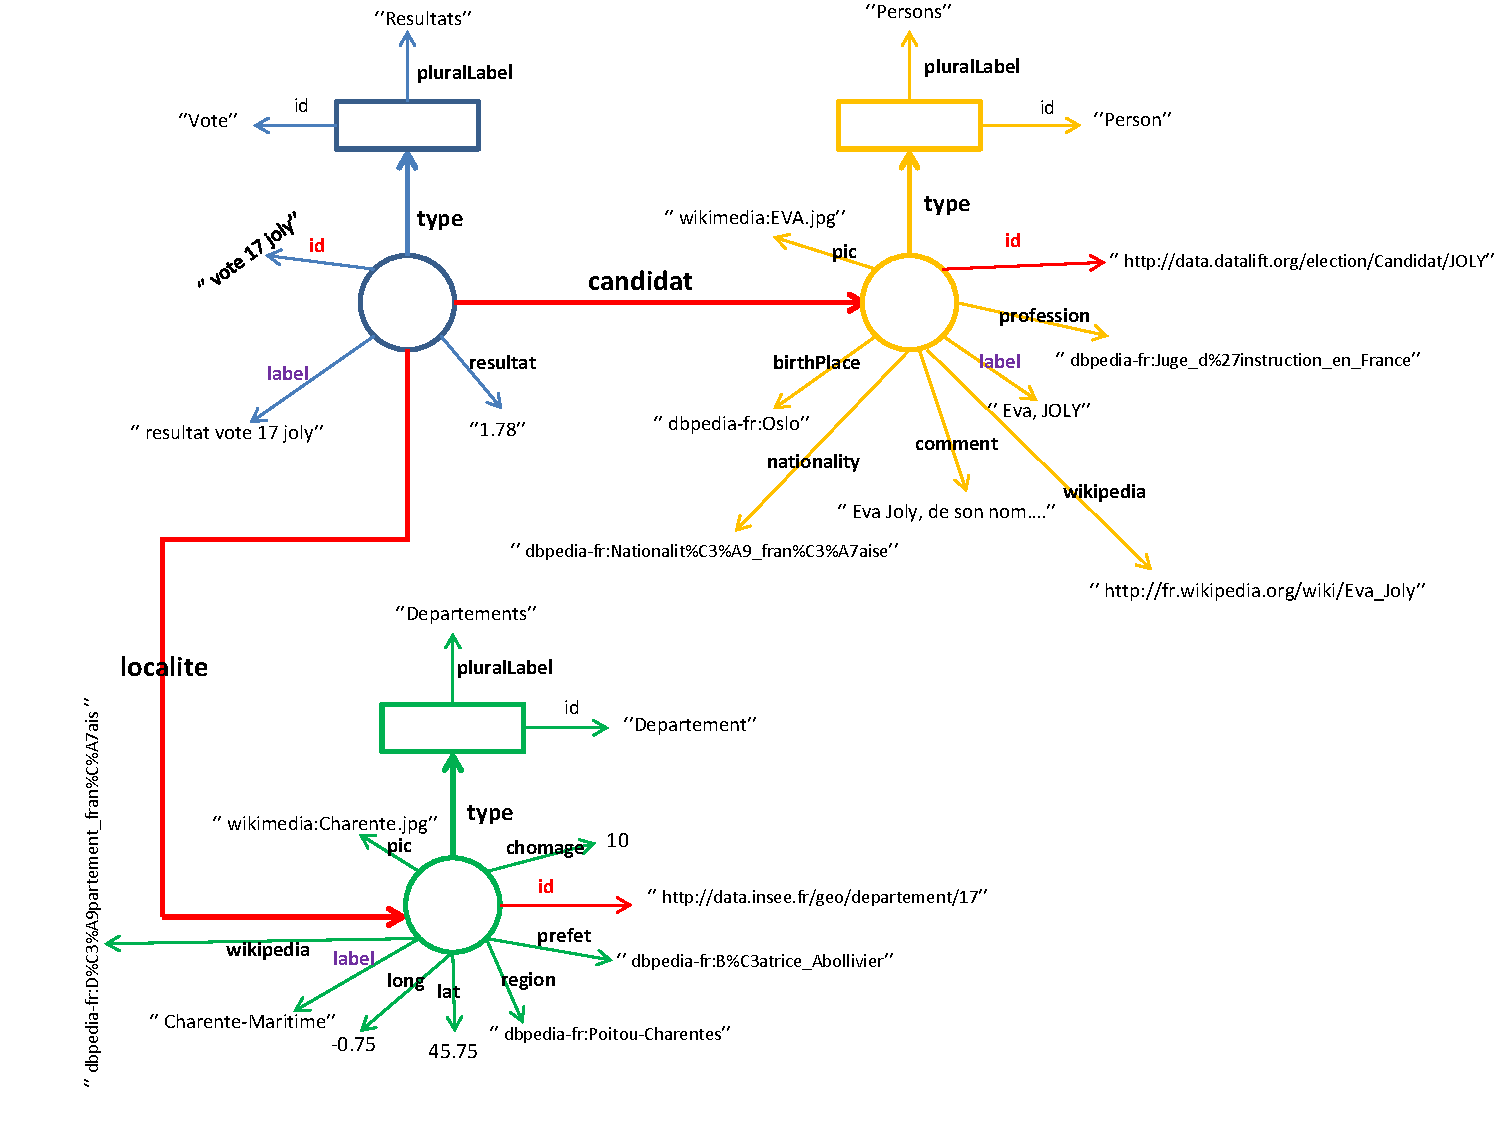
\includegraphics[height=5in]{model_EvaJoly_data}
    \else
      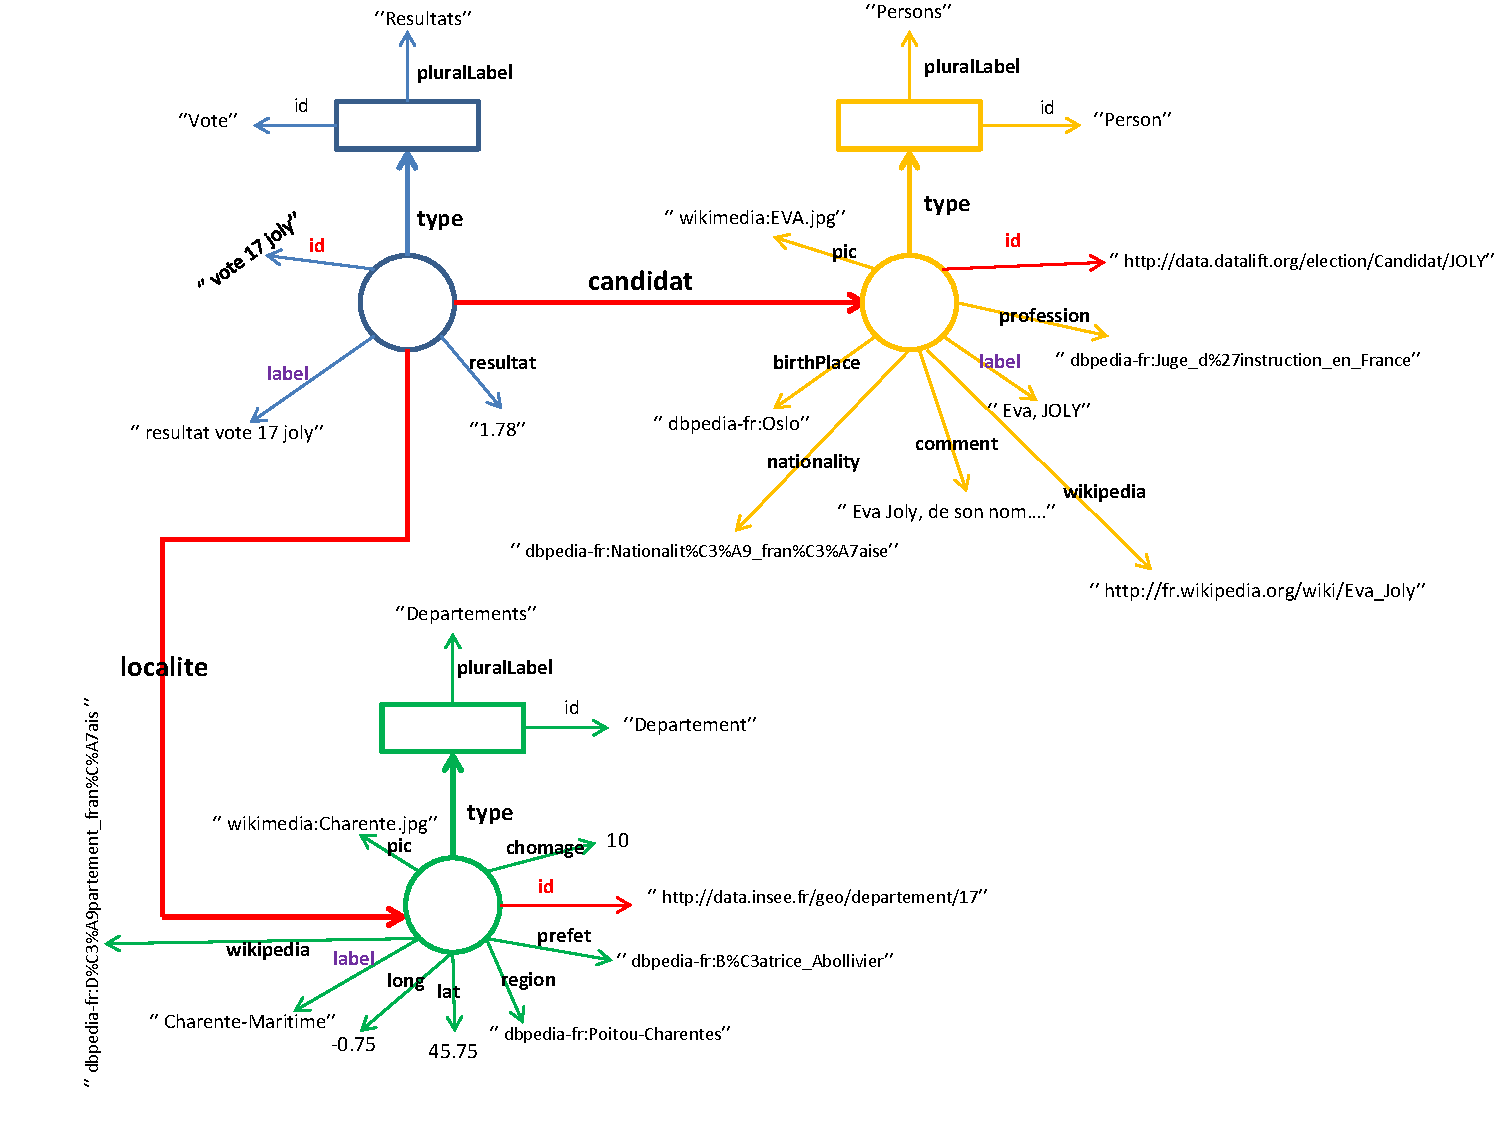
\includegraphics[bb = 92 86 545 742, height=6in]{model_EvaJoly_data}
    \fi
    \caption{Exhibit Data model of the score obtained by candidate Eva Joly in Charente-Maritime, linked with knowledge from DBpedia, INSEE and Wikipedia. }
    \label{sampleModel}
  \end{center}
\end{figure}
\end{landscape}

Regarding tools used for visualization, we have divided them into two categories, providing for each of them relevant examples: (i)-tools that operate over RDF data, and (ii) tools that operate over other structured format. We then provide some basic criteria for assessing a given visualization tool, with some weight attached to each of the criterion. 

%%%%%%%%%%%%%%%%%%%%%%%%%%%%
%%%  Section:Usage Scenarii for Application  %%%
%%%%%%%%%%%%%%%%%%%%%%%%%%%%

 \section{Usage Scenarii for Application}
 The most interesting use cases for Government Open Data are the ones which show the added value of having interconnected datasets. The need for interlinking data is almost never spontaneously expressed by the actors in France. During our interviews, only a few of them did express it, namely CG 33\footnote{\url{http://datalocale.fr}}, Etalab\footnote{\url{http://www.etalab.gouv.fr}} and Montpellier\footnote{\url{http://opendata.montpelliernumerique.fr}}. However, what is expressed, is the desire for interoperability and ease of cross-linking. Interoperability allows developers to not duplicate efforts, thus for example not duplicating a connector each time one is changing his geographical region. We list in \cite{deliverable2012a} ten key functionalities expected from the users and actors/providers of Open Data in France. It is clear that there exits some business needs that can be summarized as:
\begin{itemize}
\item \texttt{Access by territory}: case of Direction of Legal Information in France\footnote{\url{http://www.dila.premier-ministre.gouv.fr/}}
\item \texttt{Access by time period}: History, genealogy ,anecdotal history (e.g: \textit{It happens someday in}..), temporal search, temporal inquiry, games, etc.
\end{itemize}
 

%%%%%%%%%%%%%%%%%%%%%%%%%%%%%%%%%%%%%
%%%  Section:Tools for Visualizing Data on the Semantic Web  %%%
%%%%%%%%%%%%%%%%%%%%%%%%%%%%%%%%%%%%%

\section{Tools for Visualizing Data on the Semantic Web}
 
We have studied a number of tools (14) used for visualizing raw data or RDF data. The main objective is to select which could be appropriate for an agile prototyping and development of an application consuming heterogeneous data. 
The study in \cite{deliverable2012b} describes each tool according to the data formats accepted as input, how the data is accessed (API or SPARQL endpoint), the programming language of the tool, the type of views available (e.g: chart, map, text, tabular, et.), the list of libraries embedded, the license and the creator (whether organization, project or a single person). The outcome of this state-of-the-art can then be used to assess in the choice of a given visualization tool, according to some criteria, such as (i) usability, (ii) visualization, (iii) data accessibility, (iv) deployment and (v) extensibility. 


%%%%%%%%%%%%%%%%%%%%%%%%%%%%%%%%%%%%%
%%%  Section:DVIA: A vocabulary   Describing VIsualization Applicatio  %%%
%%%%%%%%%%%%%%%%%%%%%%%%%%%%%%%%%%%%%

\section{DVIA: A vocabulary   Describing VIsualization Application}
DVIA is a small vocabulary aims at describing any applications developed to consume datasets in 4-5 stars, using visual tools to showcase the benefits of Linked Data. It reuses four existing vocabularies: \texttt{Dublin Core terms} \footnote{\url{http://purl.org/dc/terms/}}, \texttt{dataset catalogue (DCAT)}\footnote{\url{http://www.w3.org/ns/dcat#}}, \texttt{Dublin Core Metadata Initiative}\footnote{\url{http://purl.org/dc/dcmitype}} and \texttt{Organization vocabulary}\footnote{\url{http://www.w3.org/ns/org#}}.  It is composed of three main classes : 

\begin{itemize}
\item \textbf{Application}: This class represents the application or the mashup developed for demo-ing or consuming data in LD fashion. It is subclass of \textbf{dctype:Software}
\item \textbf{Platform}: The platform where to host or use the application, could be on the web (Firefox, chrome, IE, etc..) or mobile (android, etc..) or event desktop
\item \textbf{VisualTool}: Represents the tool or library used to build the application. 
\end{itemize}

The diagram of the main classes and properties is depicted in Figure \ref{visuGraphModel}. The goal is to test the vocabulary with all the finalists applications submitted at the Semantic Web Challenge in  the two previous years (2011-2012). The actual version of the vocabulary in turtle format can be found here http://www.eurecom.fr/~atemezin/datalift/visumodel/visu-vocab.ttl directory, along with a sample description of the application which won the Semantic Web Challenge\footnote{url{http://challenge.semanticweb.org/2012/winners.html}} this year\footnote{\url{http://www.eurecom.fr/~atemezin/datalift/visumodel/eventMedia-sample.ttl}}.

\begin{landscape}
\begin{figure}[!htbp]
  \begin{center}
    %\leavevmode
    \ifpdf
      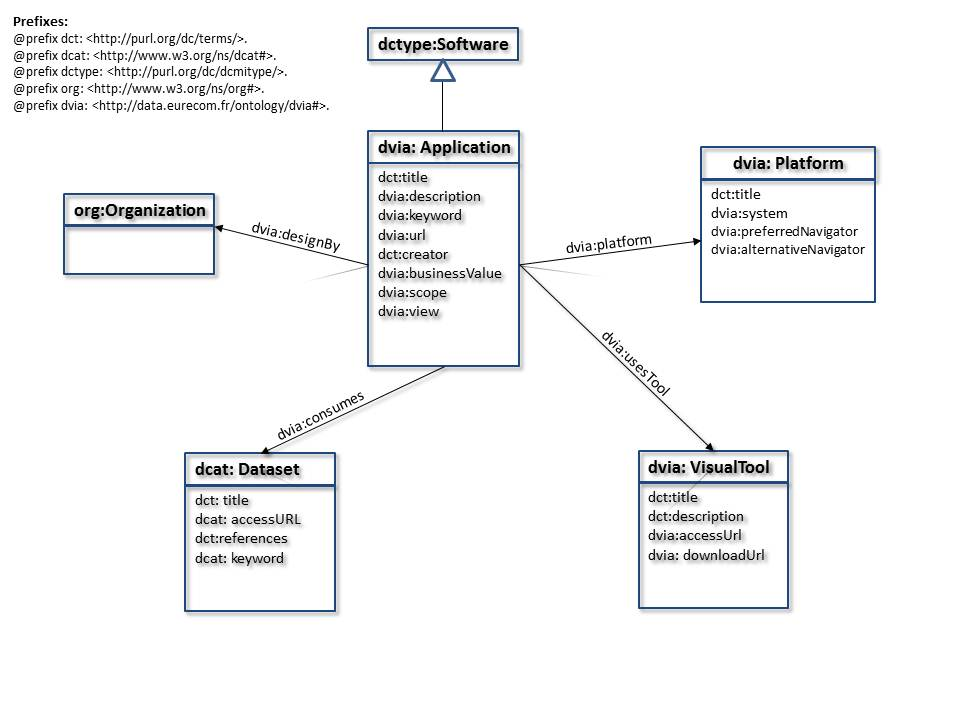
\includegraphics[height=5in]{visuGraphModel.jpg}
    \else
      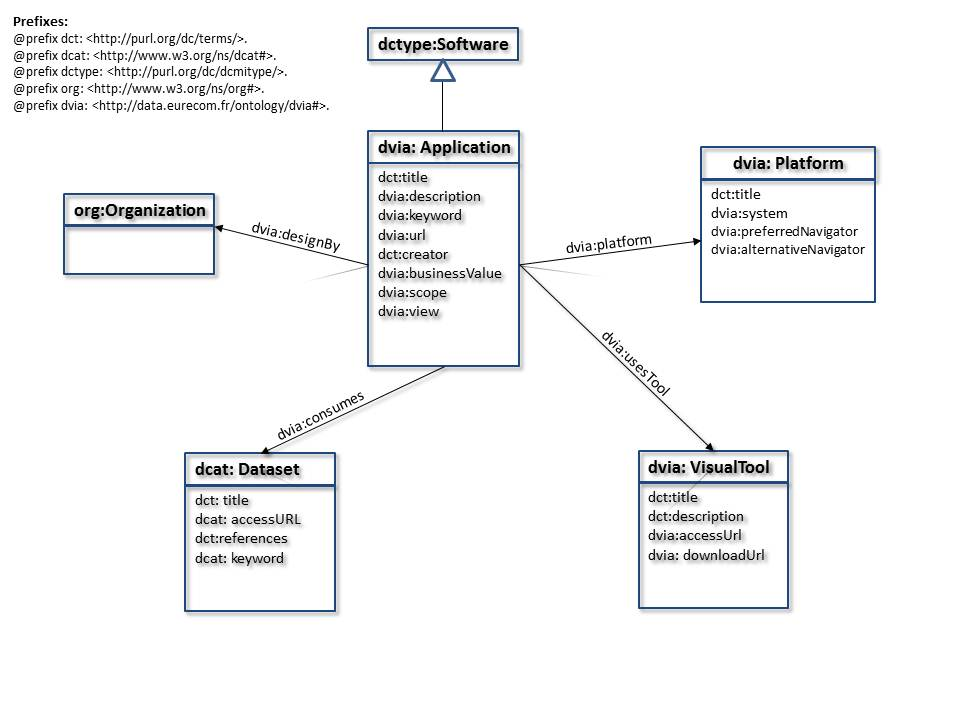
\includegraphics[bb = 92 86 545 742, height=6in]{visuGraphModel.jpg}
    \fi
    \caption{Conceptual Model of the DVIA vocabulary }
    \label{visuGraphModel}
  \end{center}
\end{figure}
\end{landscape}



\section{Examples of Visualization}
We had the opportunity to use some of the tools described in \cite{deliverable2012b} to build some innovative applications using heterogeneous data exposed as RDF. We describe two of them in the following subsections.
 
\subsection{French Election Application}
The application was built to showcase the use of a visualization application of top of heterogeneous government data exposed in RDF.
Election\footnote{\url{http://www.eurecom.fr/~atemezin/DemoElection/}} is a mashup implemented in Exhibit using four datasets: the first results of presidential election in France, the rate of unemployment by INSEE,
fr.dbpedia (http://fr.dbpedia.org/), dbpedia.org and geolocation data of districts and regions by IGN. The application provides means to search by a picture of 
a candidate, and make use of filters representing five dimension facets (candidate, region, department, rate of vote, rate of unemployment) to depict on 
a map centered to France, the appropriate results, along with more relevant details about the candidate, the description of the region, etc... Figure \ref{sampleModel} shows 
a sample of the data model follows to implement the back-end of the application.   


\subsection{Confomaton Application}
Confomaton \cite{khrouf-eswc2012} is a semantic web application that aggregates and reconciles information such as tweets, slides, photos and videos shared on social media that could potentially be attached to a scientific conference. The main demonstrator is available at \textit{http://eventmedia.eurecom.fr/confomaton} reflecting the up-to-date conferences coming from Lanyard feeds. A second demonstrator corresponding to the archived of ISWC 2011 conference \cite{khrouf-ramms12} is available at http://eventmedia.eurecom.fr/iswc2011. The user interface for the aforementioned demonstrators is built around four perspectives (tabs in the UI) characterizing an event: \textit{(i) Where does the event take place?}, \textit{(ii) What is the event about?},  \textit{(iii) When does the event take place?}, and finally \textit{(iv) Who are the participants of the event?}. Those four perspectives correspond to views in the Confomaton API configuration. 

 %\section{Towards a Framework For Generating Automatically Visualizations From Linked Data}
  %\subsection{Requirements}
  %\subsection{Specifications}
  %\subsection{Implementation}



   

%%%%%%%%%%%%%%%%%%%%%%%%%%%%%%%%%%%%
%%%  Conclusions and Future Work %%%
%%%%%%%%%%%%%%%%%%%%%%%%%%%%%%%%%%%%

\chapter{Conclusions and Future work}

We have presented in this document our main contributions in some issues around publishing and consuming Government Linked Data on the Semantic Web. We have first focus on geographic data, proposing some best practices to take into account for better interoperability of features and geometry.
We apply our propositions on the French domain, starting from existing vocabulary to mapping with other similar vocabularies. The goal is to leverage the alignment of the dataset generated with other providers in the LOD cloud. In the second part of the document, we have studied scenarii and tools 
be used for creating visual applications to better get insights of the data. We propose a small vocabulary to describe visualization applications as a first step to formally describe as much as possible applications developed in top of government datasets, to improve their re-usability. However, we have many challenges to tackle in the following months to achieve all the goals of our problematic.       

Regarding the geodata modeling, our future work includes the conversion and publication of a large RDF dataset of geographic information of the French territory together with alignments with other datasets at the instance level. At the same time, we plan to publish with IGN a new version of an adequate ontology for describing features and geometry according some best practices we are contributing to elaborate. Furthermore, some alignments with the new OGC standard GeoSPARQL will be performed and evaluated.

Regarding the visualization tools, some further studies should be made for mobile applications, as they are not considered in this current study. We plan also to develop a small vocabulary that could be used to describe OpenData applications. At the same time, we will develop  more applications using different datasets for detecting patterns for visualizing RDF data. For this challenge, we will need to study the underlying data (list of properties, number of triples, categories, etc.), the ontologies used, the templates or libraries for visualizations (Exhibit, GeoAPI, LDA, Sparkl, d3.js,etc) and finally the effort for a user to build the application. This could lead to a framework for generating automatically visualizations from heterogeneous datasets extracting relevant features by data mining techniques. 

We also plan to expose as RDF some relevant applications submitted at the Semantic Web Challenge the past ten years using the DVIA vocabulary. The idea is to have a hub of a dataset describing the tools, datasets, etc.  used to build  applications consuming 4-5 stars datasets.


\nocite{*}
\bibliographystyle{amsplain}
\bibliography{biblio}

%\appendix
%\cleardoublepage
%\addcontentsline{toc}{chapter}{Annexes}


\end{document}